\documentclass[bachelor, och, pract]{SCWorks}
\usepackage[T2A]{fontenc}
\usepackage[utf8]{inputenc}
\usepackage{graphicx}
\usepackage[sort,compress]{cite}
\usepackage{amsmath}
\usepackage{amssymb}
\usepackage{amsthm}
\usepackage{fancyvrb}
\usepackage{longtable}
\usepackage{array}
\usepackage[english,russian]{babel}
\usepackage{minted}
\usepackage{tempora}
\usepackage{titlesec}
\usepackage[colorlinks=false]{hyperref}
\usepackage{xcolor}
\usepackage{hyperref}

\definecolor{linkcolor}{HTML}{799B03} % цвет ссылок
\definecolor{urlcolor}{HTML}{799B03} % цвет гиперссылок

\hypersetup{pdfstartview=FitH,  linkcolor=linkcolor,urlcolor=urlcolor, colorlinks=true}

\hypersetup{ %содержание
colorlinks,
citecolor=black,
filecolor=black,
linkcolor=black,
urlcolor=black
}
\theoremstyle{remark}
\newtheorem{theorem}{Теорема}
\newtheorem{definition}{Определение}
\newtheorem{comment}{Замечание}

\begin{document}
    \hfill \break
    \hfill \break
    \hfill \break
    \hfill \break
    \hfill \break
    \hfill \break
    \hfill \break
    \hfill \break
    \hfill \break
    \hfill \break
    \hfill \break
    \hfill \break
    \begin{center}
        \Huge Лекции по Технологиям программирования
    \end{center}
    \hfill \break
    \hfill \break
    \hfill \break
    \hfill \break
    \hfill \break
    \hfill \break
    \hfill \break
    \hfill \break
    \hfill \break

    \begin{center} Сверстал: Кузякин Никита Александрович \end{center}
    \begin{center} По лекциям ФПМИ \end{center}
    \begin{center}Плейлист с лекциями "--- \href{https://www.youtube.com/watch?v=XjGbg-N4sQc&list=PL4_hYwCyhAvaTVSzXsvFQlb-FmNqUNkPT}{тут}\end{center}
    \thispagestyle{empty} % выключаем отображение номера для этой страницы
     
    \newpage
    \tableofcontents

    \section{Принципы SOLID}
    
    \begin{itemize}[label=$\bullet$]
        \item \textbf{S} (Single Responsibility Principle) "--- один класс одна ответсвенность. Одна задача выполняется одним классом, и один класс выполняет одну задачу.
        \item  \textbf{O} (Open-Closed Principle) "--- програмные сущности должны быть открыты для расширения и закрыты для изменнеия.
        \item  \textbf{L} (Liskov Substitution Principle) "--- объекты в программе должны быть заменяемы их подтипами (дочерними классами) поведение не должно нарушиться.
        \item \textbf{I} (Interface Segregation Principle) "--- много различных интерфейсов для разных клиентов (к примеру, десктоп и мобильный клиет) лучше, чем один общий интерфейс.
        \item \textbf{D} (Dependency Inversion Principle ) "---  зависимости нужно строить на абстракциях, а не на реализациях. Если есть объект A, он реализовывает интерфейс А', и есть объект B и он реализует интерфейс B',то объекты A и B должны взаимодействовать по средствам интерфейсов A' и B'. К примеру: есть светлая и темная цветовая тема, а также операционные системы windows и linux. У нас должно быть 2 класса тема и операционная система. Интерфейс темы должен возвращать цвета соответствующей темы (темной или светлой), а интерфейс операционной системы должен возвращать фигуры, которые должны отрисовываться для иконок. Эти иконки будут получать цвет из интерфейса темы. 

        Если бы мы строили зависимость на реализациях, то нам бы пришлось писать 4 варианта реализации: светлая тема windows, светлая тема linux, темная тема windows, темная тема linux.  
    \end{itemize}
    
    \begin{theorem} 
        \textbf{Закон Деметры} "---  у нас есть объекты A, B, C. A имеет доступ к B, а B к C. Тогда объект A не должен иметь доступ к объекту C на прямую. Если объекту A нужна информация об объекте C, он должен обратиться к объекту B и получить от него информацию о C. 
    \end{theorem}



    
    \section{Архитектура ПО}
    
    \hfill \break
    \textbf{Критерии архитектуры ПО}

    \begin{itemize}[label=$\bullet$]
        \item Надежность "--- востребованей программа, которая более стабильна. К примеру, одна программа работает за 2 секунды, но раз в 10 секунд выдает неправильный результат, и есть другая программа, которая работает 5 секунд, но всегда выдает верный результат. Вторая программа будет востребованей первой.
        \item Безопасность "--- чем сложнее получить чужие пользовательские данные из ПО, тем оно лучше. Важно разделять важные данные и неважные, не нужно делать оптимизации ради оптимизаций. К примеру, не нужно шифровать информацию о том, сколько человек провел времени в приложении. 
        \item Производительность "--- чем производительней ПО, тем лучше. 
        \item Масштабируемость "--- ПО должно быть легко масштабируемой. Те легко расширяемой для большего числа пользователей, по числу запросов, по числу хранимой информации и тд.
        \item Гибкость "--- чем проще вносить изменения и устранять ошибки в системе (меньше модифицировать смежные подсистемы), тем лучше.
    \end{itemize}

    \hfill \break
    \textbf{Критерии хорошей проектировки архитектуры ПО}

    \begin{itemize}[label=$\bullet$]
        \item Масштабируемость процесса разработки "--- если вы пишете ПО не один, то чем лучше будет организован план разработки и совместных релизов, тем продуктивней будет написание кода.
        \item Тестируемость "--- нужно заранее придумать как будет тестироваться ПО. К примеру, позаботиться о тестах с большими данными или тестах на пользователях из разных регионов.
        \item Возможность повторного использования "--- хорошо написанная подсистема должна легко интегрироваться в другие проекты, при этом для ее работы не нужно переносить смежные блоки в новый проект.
        \item Сопровождаемость "--- перед написанием ПО нужно задуматься о том: как оно будет обновляться, как вы будете получать bug report (отчет об ошибках) от пользователя, как быстро вы сможете исправить ошибки у пользователя.
    \end{itemize}

    \hfill \break
    \textbf{Критерии хорошей проектировки архитектуры ПО}

    \begin{itemize}[label=$\bullet$]
        \item Масштабируемость процесса разработки "--- если вы пишете ПО не один, то чем лучше будет организован план разработки и совместных релизов, тем продуктивней будет написание кода.
        \item Тестируемость "--- нужно заранее придумать как будет тестироваться ПО. К примеру, позаботиться о тестах с большими данными или тестах на пользователях из разных регионов.
        \item Возможность повторного использования "--- хорошо написанная подсистема должна легко интегрироваться в другие проекты, при этом для ее работы не нужно переносить смежные блоки в новый проект.
        \item Сопровождаемость "--- перед написанием ПО нужно задуматься о том: как оно будет обновляться, как вы будете получать bug report (отчет об ошибках) от пользователя, как быстро вы сможете исправить ошибки у пользователя.
    \end{itemize}
    
    \hfill \break
    \textbf{Критерии плохой архитектуры }

    \begin{itemize}[label=$\bullet$]
        \item Жесткость "--- тяжело изменить
        \item Хрупкость "--- изменения нарушают работу других систем.
        \item Неподвижность "--- тяжело извлечь(удалить) модули(данные).
    \end{itemize}

    \begin{definition}
        \textbf{Сильная сопряженность внутри модуля (High Cohesion)} "--- внутри модуля должны находиться только сильно сопряженные подсистемы. Слабо сопряженную подсистему лучше всего вынести за модуль, благодаря этому при обновление не придется затрагивать ее или модуль. 
    \end{definition}

    \begin{definition}
        \textbf{Low Coupling} "--- Модули независимые друг от друга слабо связаны. Можно сказать, что модули представляют собой компоненты сильной связанности. Тогда принцип Low Coupling, говорит о том, что между этими компонентами должно быть как можно меньше мостов(связей).
    \end{definition}

    
    
    \begin{comment}
        \textbf{Обещать что-то пользователю нужно аккуратно, а то он и напомнить может.}
    \end{comment}
    
    \section{Методы отладки ПО}
    \textbf{Категории ошибок:}
    \begin{itemize}[label=$\bullet$]
        \item критичные
        \item срочные
        \item несрочные
        \item "особенности реализации"
    \end{itemize}

    \textbf{Что нужно делать после отладки?} Проверить, что ошибка исправлена у вас, проверить точно ли ошибка исправлена у клиента.
  

    \textbf{Критерии критичности ошибок:}
    \begin{itemize}[label=$\bullet$]
        \item какой процент пользователей пострадал
        \item на сколько большая часть приложения не работает
        \item происходит ли порча (потеря) данных
        \item сложность обхода
    \end{itemize}


    \subsection{Воспроизведение дефекта}
    Суть данного этапа заключается в том, что нужно поймать точно такую же ошибку, которая возникла у пользователя,а не просто завершить программу с ошибкой. 

    \textbf{Порядок воспроизведение дефекта}
    \begin{enumerate}
        \item Проверка соответствия версия ПО с ошибкой и ваша.
        \item Проверка соответствуют ли настройки ПО с ошибкой и ваша.
        \item Проверка соответствуют ли данные ПО с ошибкой и ваша.
        \item Точное воспроизведение действий пользователя (сценария ошибки).
    \end{enumerate}
    
    
    Для быстрой проверки этих данных нужно тщательно собирать логи ошибок.

    \begin{comment}
        По умолчанию пользователь не хочет обновляться.
    \end{comment}


    \subsection{Анализ дефекта}

    \begin{definition}
        \textbf{Root Cause (суть проблемы)} "--- нужно исправлять не следствия ошибки, а саму суть. К примеру, если у вас выводится неправильно сумма 10 + 15, то нужно исправлять функцию суммирования, а не конкретно сумму для этих двух чисел. 
    \end{definition}

    \textbf{Условия возникновения} "--- когда происходит ошибка, нужно проверить все смежные сценарии.
    
    \textbf{Область повреждения} "--- ошибка в одном месте может сломать огромное количество сценариев.

    \textbf{Кто привнес ошибку} "--- имея такие данные можно понять, какие именно системы требуют более тщательного контроля, каких тестов нехватает и тд.

    \subsection{Дизайн исправления дефекта}
    \textbf{Технический дизайн} "--- как ошибка будет исправлена в коде.
    
    \textbf{Архитектурный дизайн} "--- внедрение новых модулей, которые смогут предотвратить появление ошибки.
    
    \textbf{Технологический дизайн} "--- stack технологий устарел, и для исправления требуется переход на новый stack технологий.

    После исправления важно провести ревью и согласование, ведь вы могли затронуть подсистемы, которые используют / редактируют другие люди.

    \subsection{Исправление дефекта}
    \begin{theorem}
        \textbf{Главное правило.} При исправление дефекта, не привнеси новые дефекты.
    \end{theorem}
    
    Не всегда ожидаемое поведение для вас и для пользователя совпадает. Поэтому важно получить обратную связь с пользователем, что его ошибка исправлена.

    Очень важно документировать все изменение в системе, особенно исправление ошибок.
    
    Перед загрузкой новой версии важно проверить все, даже те вещи, которые не менялись, даже на старых тестах и тд. Те происходит полноценное тестирование системы. 

    Также важно проверить корректность обновления.

    \begin{comment}
        \textbf{Иногда сложность исправления ошибки на столько велика, что проще сказать пользователю путь обхода ошибки.}
    \end{comment}
    

    \subsection{Техники отладки}
    
    \hfill \break
    \textbf{Запуск в отладчике}
    
    Самый простой способ это запуск программы в отладчике.
    
    Виды отладкиков:
    \begin{itemize}[label=$\bullet$]
        \item софтверный (как в visual studio, pycharm).
        \item "железный" "--- подключается напрямую к системе, на которой выполняется процесс и выводит данные на ваше устройство.
        \item Удаленный дебагер "--- посылает данные на ваше устройство с устройства, на котором происходит задача (к примеру, сервер посылает данные на локальную машину).
    \end{itemize}

    \hfill \break
    \textbf{Анализ кода, без запуска программы}

    Данный метод заключается в анализе кода, без запуска программы. Нужно самому понять к чему приводят вызовы процедур, в каком порядке они выполняются и тд.
   
    \hfill \break
    \textbf{Анализ поведения программы}

    Данный метод заключается в построение причинно следственных связей для поиска ошибки. Делается предположение о причине ошибки, отталкиваясь от него делается предположение о сути ошибки и тд, пока вы не добираетесь для корня проблемы. Также в данном методе применяют упрощение сценариев тестирования и уменьшения данных, на которых тестируется ПО.

    Данный метод помогает локализовать ошибку в крупных системах.
    
    \hfill \break
    \textbf{UNIT - тестирование}
    
    Предполагает тестирование каждой отдельной функции или каждого элемента системы.

    \begin{definition}
        \textbf{Процент покрытия кода} "--- процент функций, на которые написаны тексты. Чем больше покрытие кода, тем лучше.
    \end{definition}

    \begin{definition}
        \textbf{Self test} "--- после установки приложение запускает тест самого себя. Что гарантирует корректность установки.
    \end{definition}

    \hfill \break
    \textbf{Прототипирование}
    
    Метод, при котором для тестировки, модуль выносится в отдельное пространство и для него дописывается минимальный набор функций для запуска. 

    Данный метод хорошо подходит в случае, когда невозможно произвести полное тестирование системы вместе с данным модулем.

    \hfill \break
    \hfill \break
    \textbf{Отадка с помощью дампов}
    
    \begin{definition}
        \textbf{Файл дампа} — это моментальный снимок, показывающий выполнявшийся процесс и загруженные для приложения модули в определенный момент времени. Дамп со сведениями о куче также содержит моментальный снимок памяти приложения на этот момент.
    \end{definition}

    В основном дампы используются для отладки проблем на компьютерах, к которым у разработчиков нет доступа. Если вы не можете воспроизвести на своем компьютере аварийное завершение или зависание программы, возникшие на компьютере клиента, вы можете записать файл дампа с его компьютера. Дампы также создаются тест-инженерами, чтобы сохранить данные для дополнительного тестирования.

    \hfill \break
    \textbf{Отладка с помощью перехватов}
    
    В данном методе, если есть предположение, что конкретная функция работает не правильно, то существуют специальные ПО, которые при вызове этой функции перехватят все передаваемые значения и тд. 

    Данный метод используется для ускорения тестировки, тк ПО в режиме дебагера работает гораздо дольше.

    \begin{definition}
        \textbf{Профилирование кода} "--- Сбор характеристик работы программы, таких как время выполнения отдельных фрагментов, число верно предсказанных условных переходов, число кэш-промахов, количество затрачиваемой оперативной памяти и т. д. 
    \end{definition}

    \begin{definition}
        \textbf{Кэш-промах (cash"= miss)} "--- Некорректная логика работы кэша. 
    \end{definition}

    \hfill \break
    \textbf{Трансляция кода}

    Метод, при котором код переносится на другой язык. К примеру с С++ на ассемблер для того, чтобы увидеть как это работает на более низком уровне. Или наоборот с ассемблера на С++, те на более высокий уровень, для того чтобы логика процесса была более очевидной.

    \hfill \break
    \textbf{Обратное движение по алгоритму} 

    Данный подход полезен, когда сценарий достаточно сложный, тк уровень сложности и вероятности ошибки растет ближе к концу кода. Соответственно, если начать отладку с конца, то вероятнее вы быстрее доберетесь до ошибки.


    \section{Проектирования ПО}
    
    \subsection{Этапы проектирование ПО}

    \begin{enumerate}
       \item формирование требований
        \item Разработка концепции 
        \item Техническое задание
        \item Эскизный проект 
        \item Технический проект
        \item Рабочая документация
        \item Поставка и ввод в действие
        \item Сопровождение
    \end{enumerate}

    \textbf{Формирование требований} "--- общение с клиентом (чаще всего сам клиент не будет пользоваться системой), общение с пользователем, анализ прикладной области, формирование оценок требуемой производительности. Важно понимать: для кого этот софт и какую проблему он решает.
    

    \textbf{Разработка концепции} "--- изучение объекта автоматизации, проведение необходимых научно"=исследовательских работ, разработка вариантов концепции. \textbf{Важно, подготовить отчетность по данному этапу}. Также тут уточняется: формат поставки (приложение андроид, веб сайт и тд), целевое оборудование (оборудование на котором должно работать ПО), выбор стека технологий.

    \textbf{Техническое задание} "--- описание системы, описание функциональности, описание требований к системе и функциональности, описание сценариев использования, условия сдачи. \textbf{Техническое задание очень важно как для программиста, так и для заказчика}. Тк заказчику оно дает гарантию того, что ПО будет выполнять все, что прописано в ТЗ. А программисту дает гарантию того, что если выполнено все ТЗ, то ПО будет принято заказчиком.

    \textbf{Эскизный проект} "--- разработка прототипов частей системы (не всех, а самых важных и сложных), тестирование, оценка производительности и качества, MVP.

    \textbf{Технический проект} "--- разработка частей системы, написание документации пользователя, тестирование, разработка заданий на проектирование и реализацию смежных систем, оценка производительности.

    \textbf{Рабочая документация} "--- описание всех сценариев использования, описание логики работы, описание производительности, примеры использования, обучающие мероприятия.

    \textbf{Ввод и действие} "--- подготовка объекта автоматизации, подготовка персонала, проведение предварительных испытаний, опытная эксплуатация, приемочные испытания (проверка всех ограничений из ТЗ).

    \subsection{UML}

    \begin{definition}
        \textbf{UML} "--- унифицированный язык моделирования (Unified Modeling Language). Это система обозначений, которую можно применять для объектно-ориентированного анализа и проектирования Его можно использовать для визуализации, спецификации конструирования и документирования программных систем.
    \end{definition}

    Основные цели дизайна UML:

    \begin{itemize}[label=$\bullet$]
        \item Предоставить пользователям готовый, выразительный язык визуального моделирования, чтобы они могли разрабатывать и обмениваться осмысленными моделями.
        \item Обеспечить механизмы расширяемости и специализации для расширения основных понятий.
        \item Быть независимым от конкретных языков программирования и процессов разработки.
        \item Обеспечить формальную основу для понимания языка моделирования.
        \item Поощрять рост рынка объектно-ориентированных инструментов.
        \item Поддержка высокоуровневых концепций разработки, таких как совместная работа, структуры, шаблоны и компоненты.
        \item Интегрировать лучшие практики.
    \end{itemize}

    Диаграммы UML подразделяют на два типа — это структурные диаграммы и диаграммы поведения.

    Структурные диаграммы показывают статическую структуру системы и ее частей на разных уровнях абстракции и реализации, а также их взаимосвязь. Элементы в структурной диаграмме представляют значимые понятия системы и могут включать в себя абстрактные, реальные концепции и концепции реализации.
    
    Диаграммы поведения показывают динамическое поведение объектов в системе, которое можно описать, как серию изменений в системе с течением времени. 

    \begin{figure}[H]
        \begin{center}
            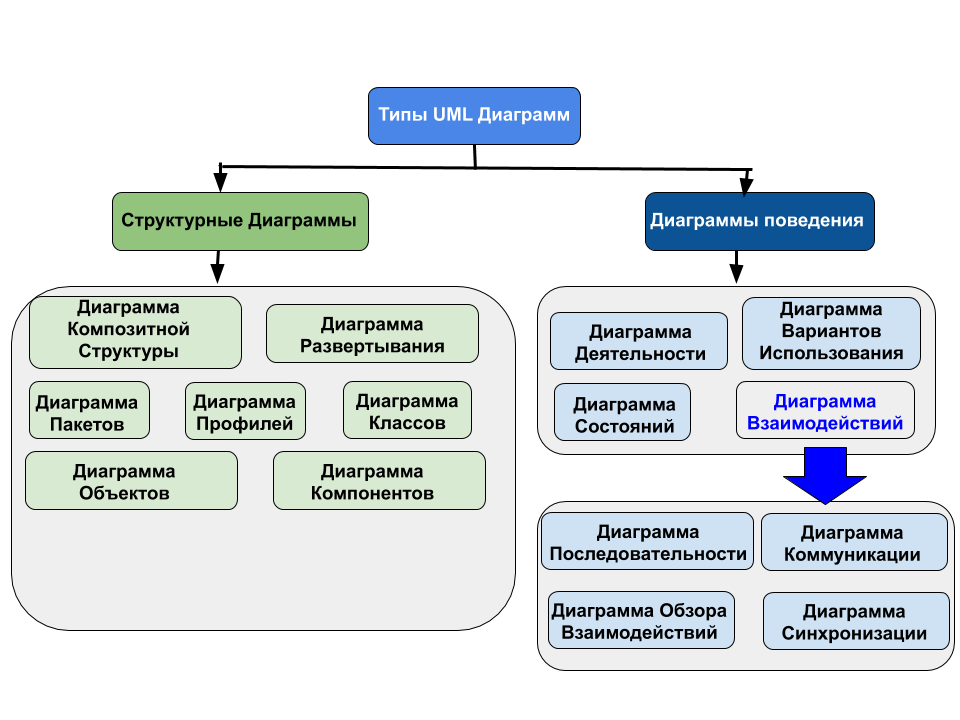
\includegraphics[scale=0.5]{res/type-uml.png}
        \end{center}
    \end{figure}


    \newpage
    \textbf{Диаграмма классов} "--- включает в себя три компонента: Ассоциация, которая представляет отношения между экземплярами типов, наследование, и агрегация, которая представляет из себя форму композиции объектов в объектно-ориентированном дизайне.

    \begin{figure}[H]
        \begin{center}
            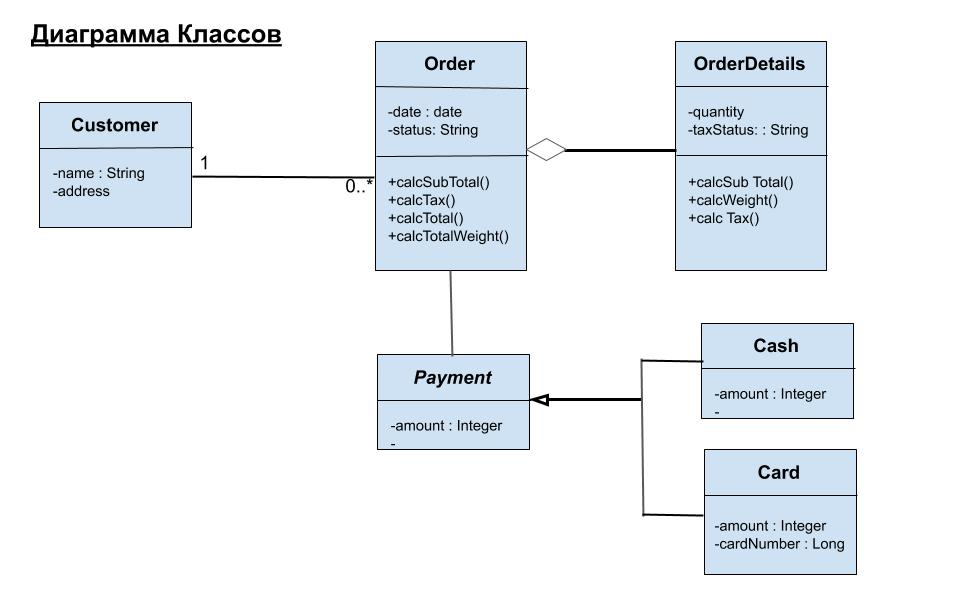
\includegraphics[scale=0.5]{res/class-diagram.png}
        \end{center}
    \end{figure}

    \newpage
    \textbf{Диаграмма компонентов} "--- показывает, как компоненты соединяются вместе для формирования более крупных компонентов или программных систем.

    \begin{figure}[H]
        \begin{center}
            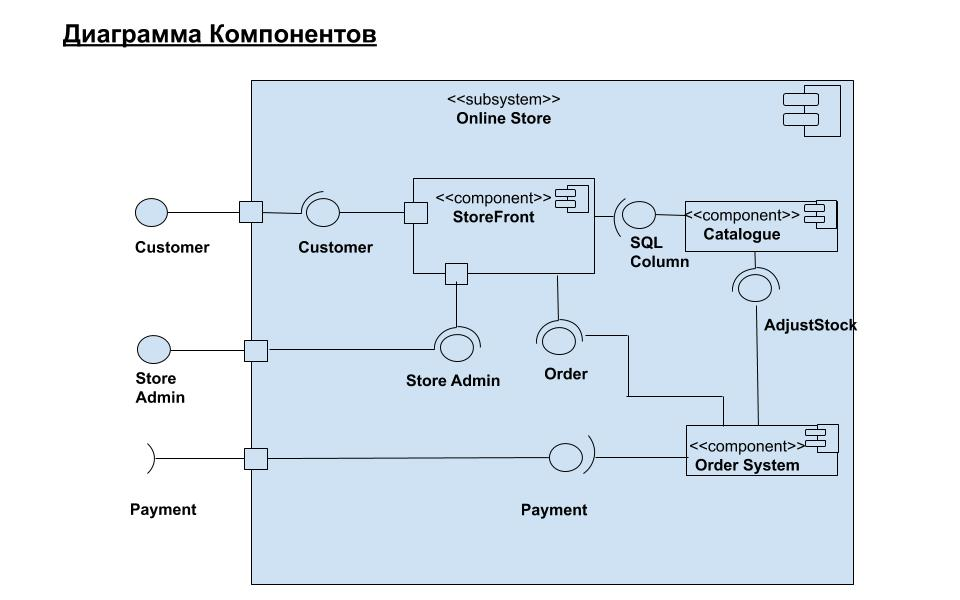
\includegraphics[scale=0.5]{res/component-diagram.png}
        \end{center}
    \end{figure}

    \newpage
    \textbf{Диаграмма развертывания} "--- показывает архитектуру системы, как развертывание (дистрибуции) программных элементов в физическом мире, которые являются результатом процесса разработки.

    \begin{figure}[H]
        \begin{center}
            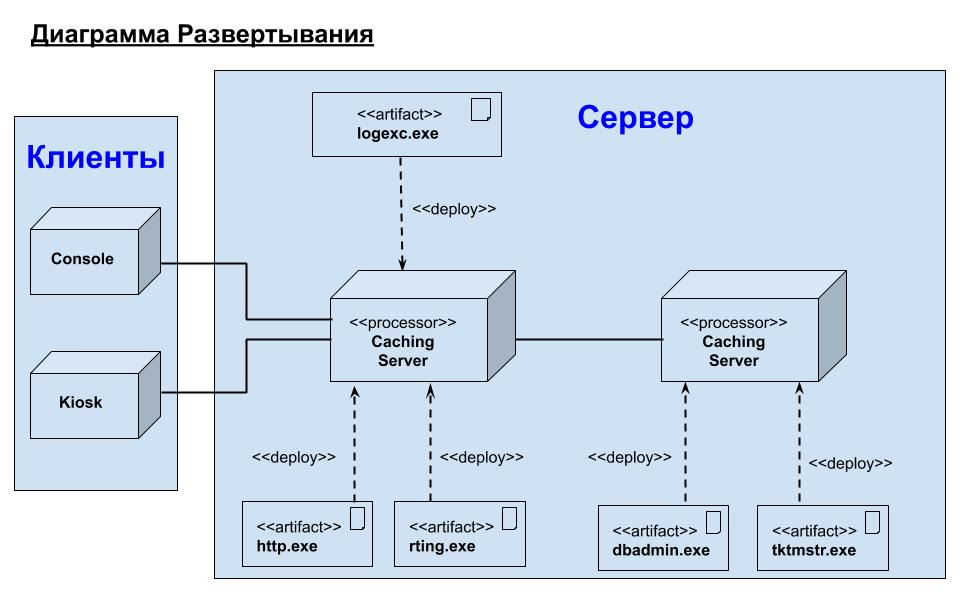
\includegraphics[scale=0.5]{res/deployment-diagram.png}
        \end{center}
    \end{figure}

    \newpage
    \textbf{Диаграмма объектов} "--- является экземпляром диаграммы класса. Она показывает снимок подробного состояния системы в определенный момент времени.

    \begin{figure}[H]
        \begin{center}
            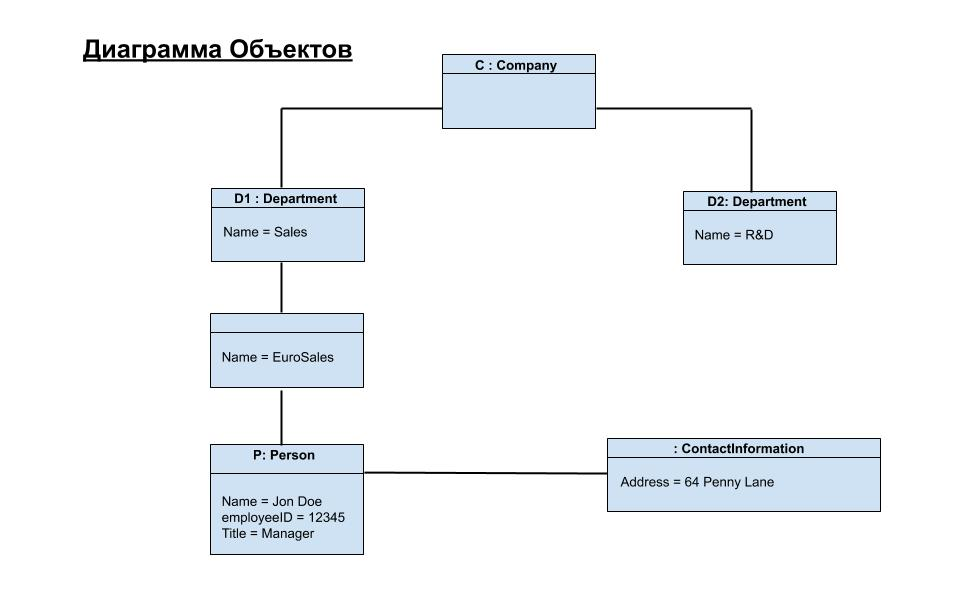
\includegraphics[scale=0.5]{res/object-diagram.png}
        \end{center}
    \end{figure}

    \newpage
    \textbf{Диаграмма пакетов} "--- это структурная схема, которая показывает пакеты и зависимости между ними.

    \begin{figure}[H]
        \begin{center}
            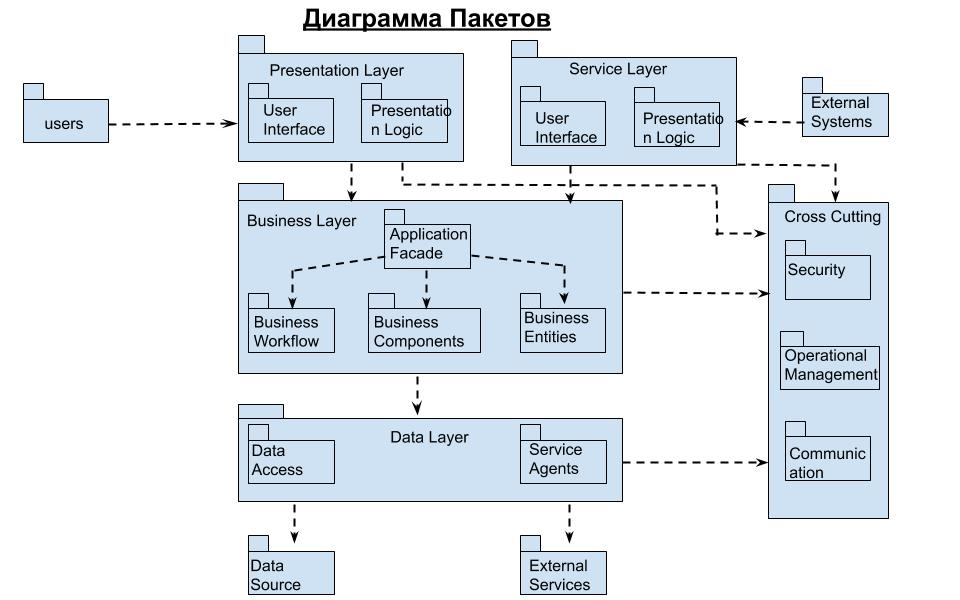
\includegraphics[scale=0.5]{res/package-diagram.png}
        \end{center}
    \end{figure}
    
    \newpage
    \textbf{Диаграмма составной структуры} "--- аналогична диаграмме классов и является своего рода диаграммой компонентов, используемой в основном при моделировании системы на микроуровне, но она изображает отдельные части вместо целых классов. Это тип статической структурной диаграммы, которая показывает внутреннюю структуру класса и взаимодействия, которые эта структура делает возможными.
    
    \begin{figure}[H]
        \begin{center}
            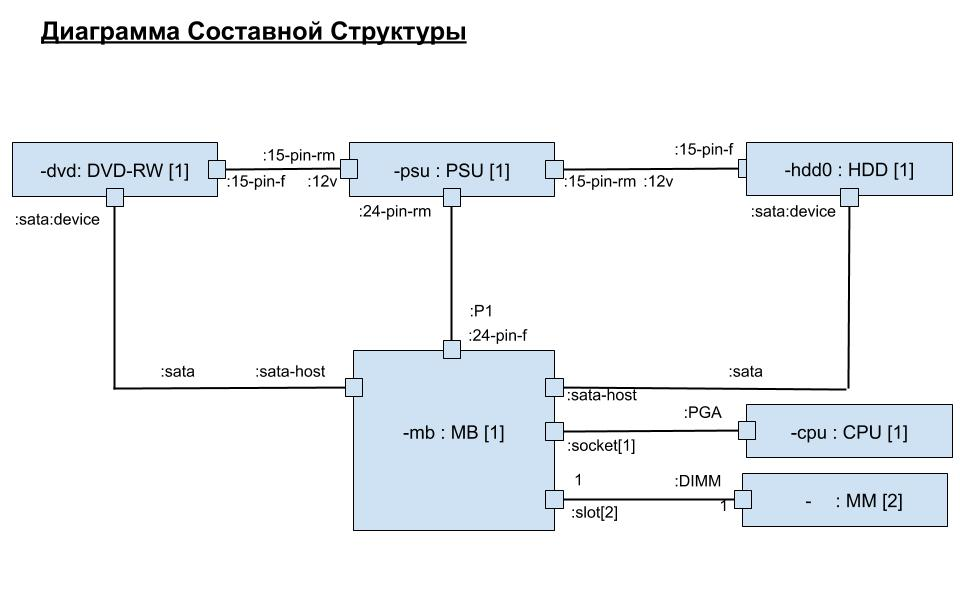
\includegraphics[scale=0.5]{res/composite-structure-diagram.png}
        \end{center}
    \end{figure}
    
    \newpage
    \textbf{Диаграмма профилей} "--- позволяет нам создавать специфичные для домена и платформы связи и определять отношения между ними. 

    \begin{figure}[H]
        \begin{center}
            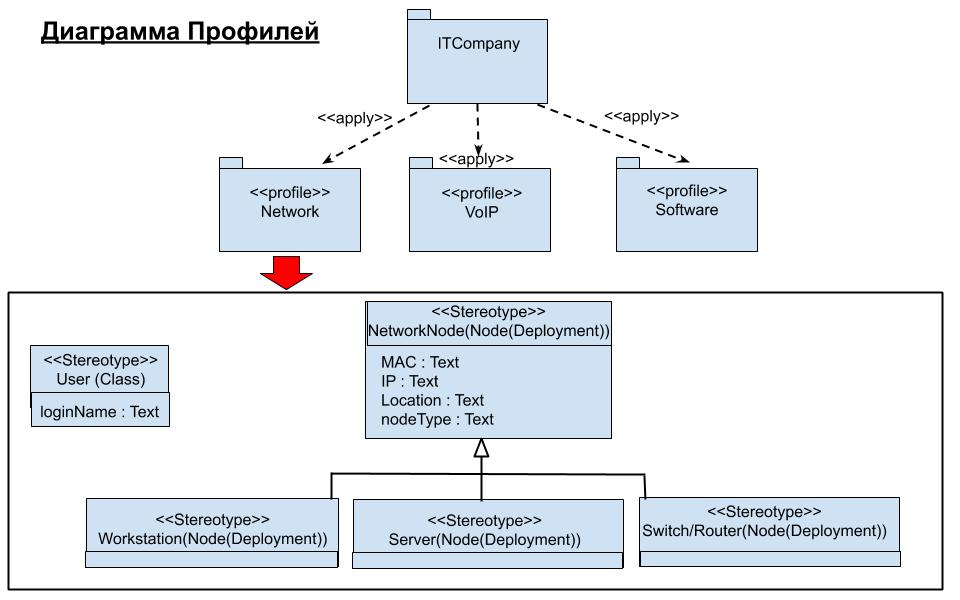
\includegraphics[scale=0.5]{res/profile-diagram.png}
        \end{center}
    \end{figure}


    \newpage
    \textbf{Диаграмма прецедентов} "--- описывает функциональные требования системы с точки зрения прецедентов. 
    
    \begin{figure}[H]
        \begin{center}
            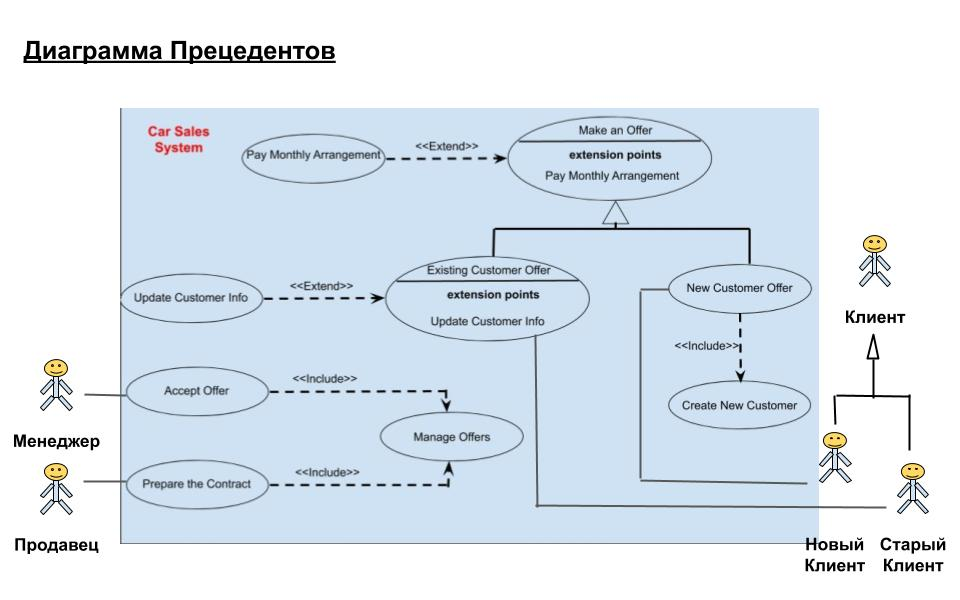
\includegraphics[scale=0.5]{res/use-case-diagram.png}
        \end{center}
    \end{figure}
    
    \newpage
    \textbf{Диаграмма деятельности} "--- представляет собой графическое представление рабочих процессов поэтапных действий и действий с поддержкой выбора, итерации и параллелизма.
    
    \begin{figure}[H]
        \begin{center}
            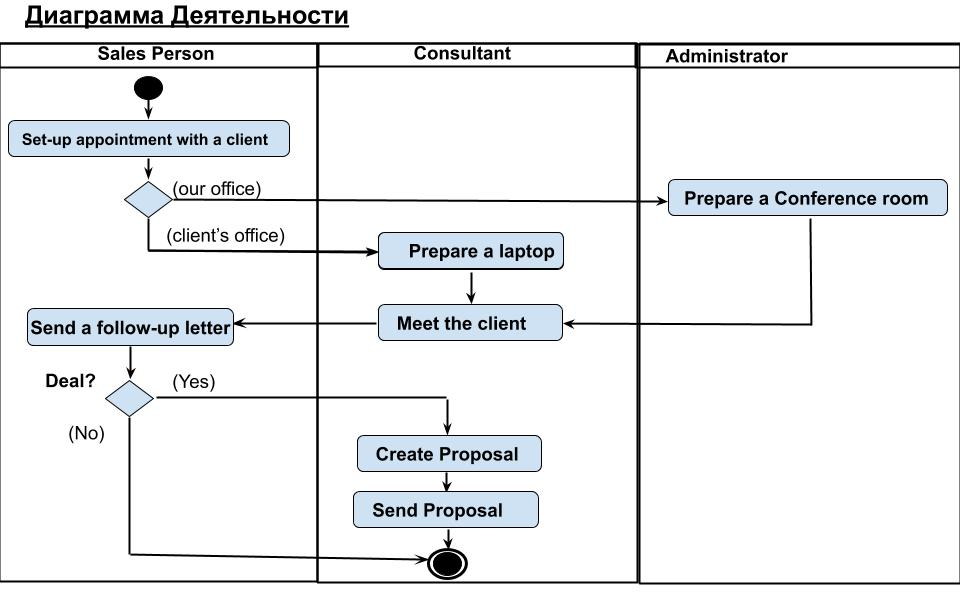
\includegraphics[scale=0.5]{res/activity-diagram.png}
        \end{center}
    \end{figure}
    
    \newpage
    \textbf{Диаграмма состояний} "--- отображает разрешенные состояния и переходы, а также события, которые влияют на эти переходы. Она помогает визуализировать весь жизненный цикл объектов.
    
    \begin{figure}[H]
        \begin{center}
            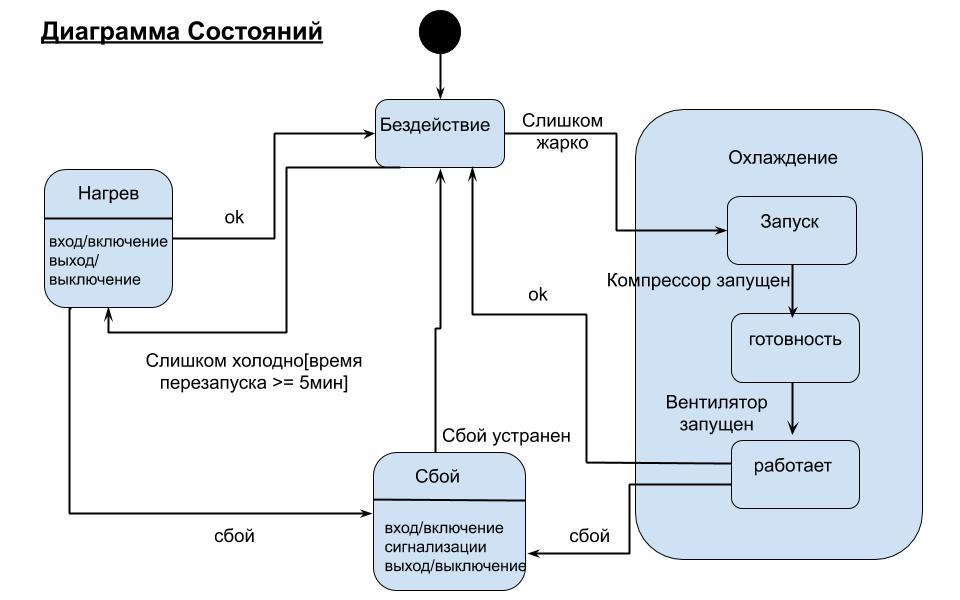
\includegraphics[scale=0.5]{res/state-diagram.png}
        \end{center}
    \end{figure}

    \newpage
    \textbf{Диаграмма последовательности} "--- моделирует взаимодействие объектов на основе временной последовательности. 
    
    \begin{figure}[H]
        \begin{center}
            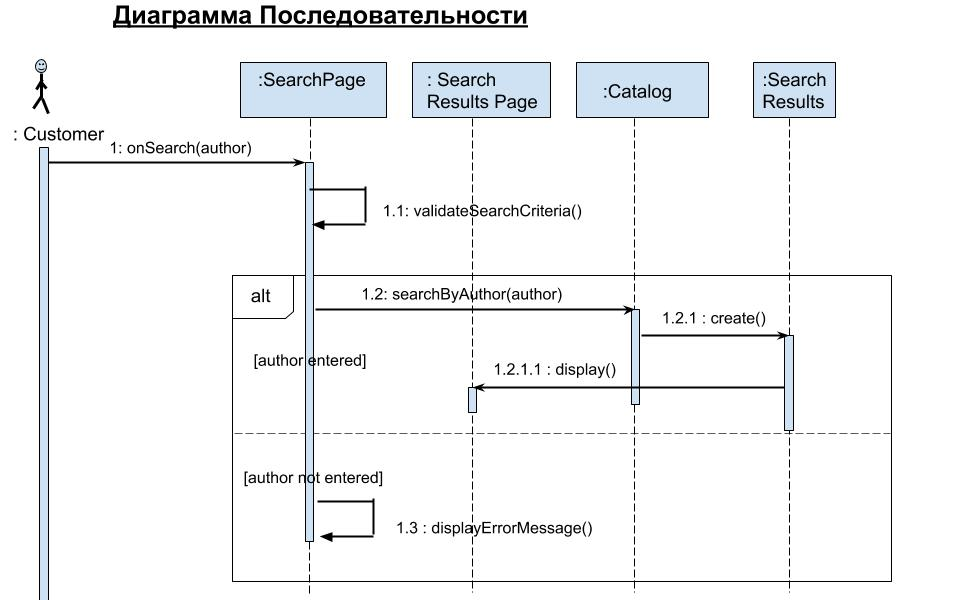
\includegraphics[scale=0.5]{res/sequence-diagram.png}
        \end{center}
    \end{figure}

    \newpage
    \textbf{Диаграмма коммуникации} "--- как и диаграмма последовательности, также используется для моделирования динамического поведения прецедента. Если сравнивать с диаграммой последовательности, Диаграмма коммуникации больше сфокусирована на показе взаимодействия объектов, а не временной последовательности. 
    
    \begin{figure}[H]
        \begin{center}
            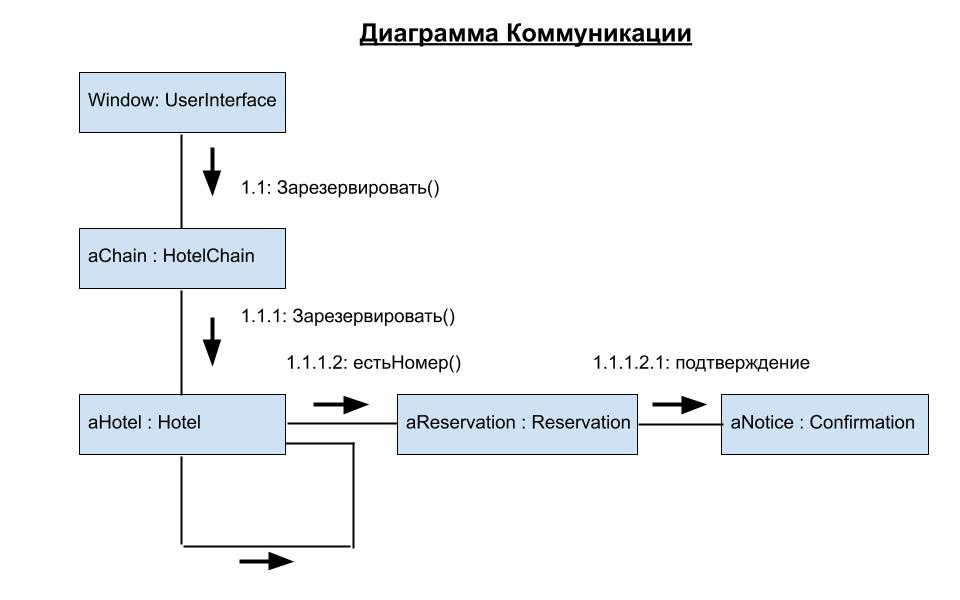
\includegraphics[scale=0.5]{res/communication-diagram.png}
        \end{center}
    \end{figure}
    
    \newpage
    \textbf{Диаграмма обзора взаимодействия} "--- фокусируется на обзоре потока управления взаимодействиями. Это вариант Диаграммы деятельности, где узлами являются взаимодействия или события взаимодействия.
    
    \begin{figure}[H]
        \begin{center}
            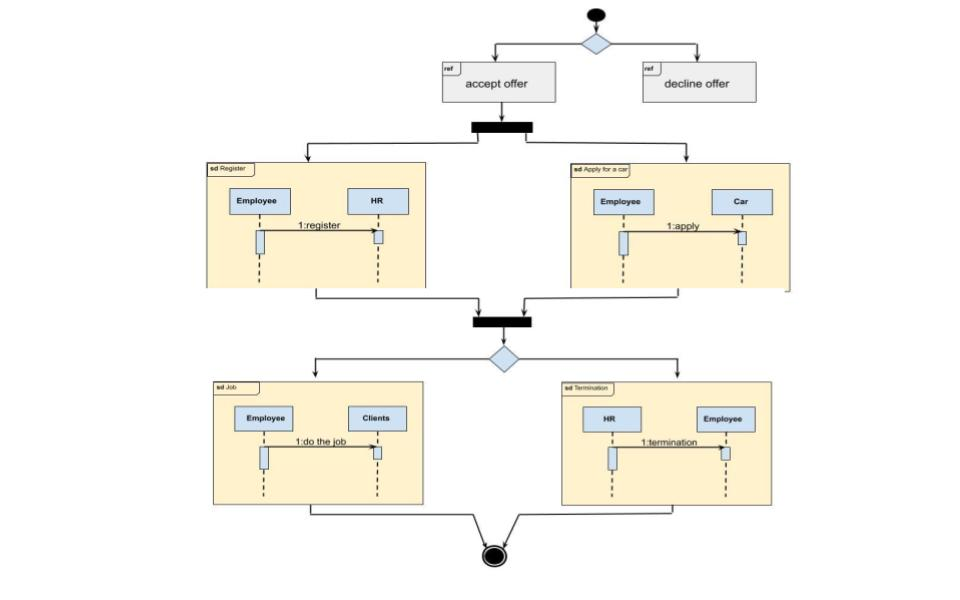
\includegraphics[scale=0.6]{res/interaction-overview-diagram.png}
        \end{center}
    \end{figure}

    \newpage
    \textbf{Временная диаграмма} "--- показывает поведение объекта в данный период времени. По сути — это особая форма диаграммы последовательности и различия между ними состоят в том, что оси меняются местами так, что время увеличивается слева направо, а линии жизни отображаются в отдельных отсеках, расположенных вертикально.

    \begin{figure}[H]
        \begin{center}
            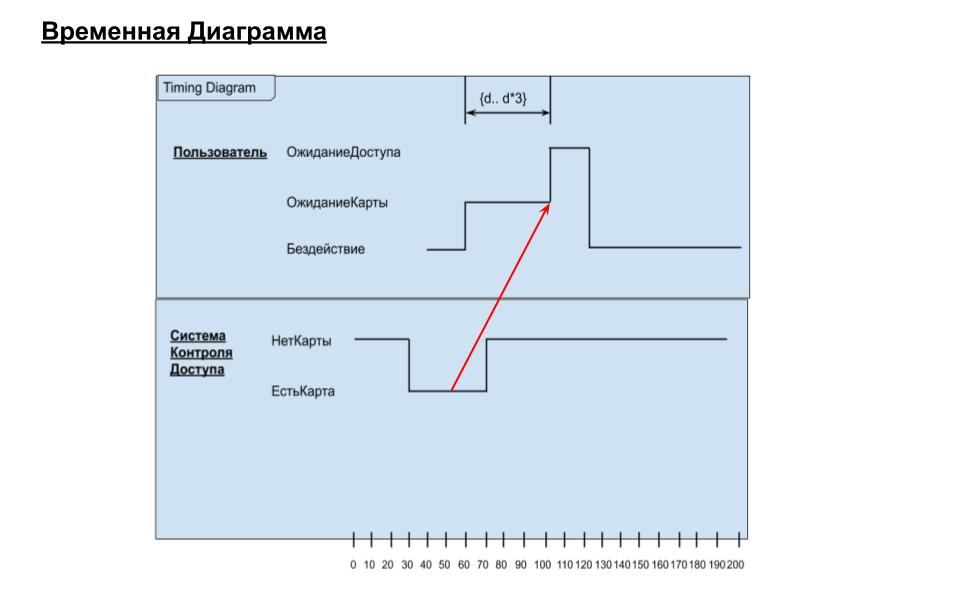
\includegraphics[scale=0.5]{res/time-diagram.png}
        \end{center}
    \end{figure}

















    
    \subsection{Методологии разработки}

    \begin{definition}
        \textbf{Методология разработки} "--- набор методов, принципов и правил, которые используются для постановки задачи, планирования, контроля и в конечном итоге — для достижения поставленной цели. 
    \end{definition}


    \begin{center}
        \textbf{Водопадная модель}    
    \end{center}

    \begin{itemize}[label=$\bullet$]
        \item все стадии проекта идут строго друг за другом
        \item следующая стадия не начинается, пока не закончится предыдущая
        \item план разрабатывается сразу на весь проект
    \end{itemize}

    \begin{figure}[H]
        \begin{center}
            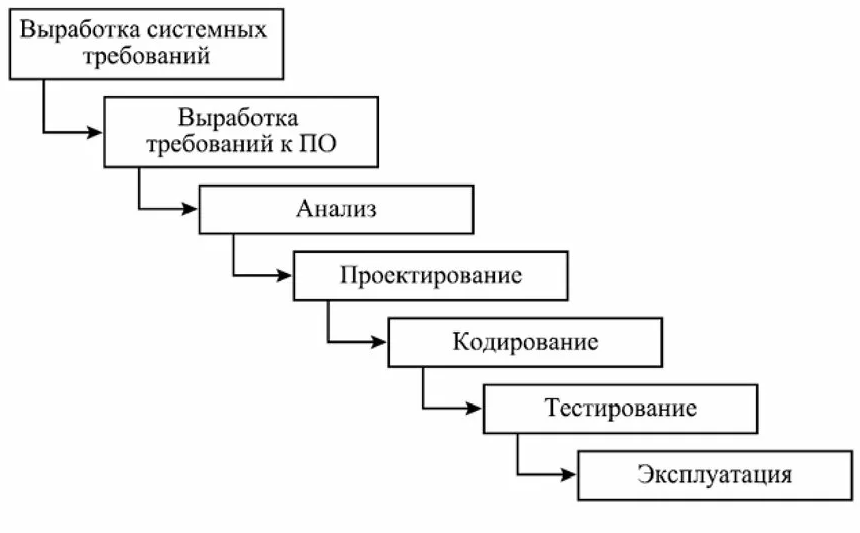
\includegraphics[scale=0.5]{res/waterfall.png}
            \caption{Водопадная модель разработки ПО}
        \end{center}
    \end{figure}

    Главный минус "--- это возможное изменение требований, что может полностью обесценить уже сделанную работу.

    \begin{figure}[H]
        \begin{center}
            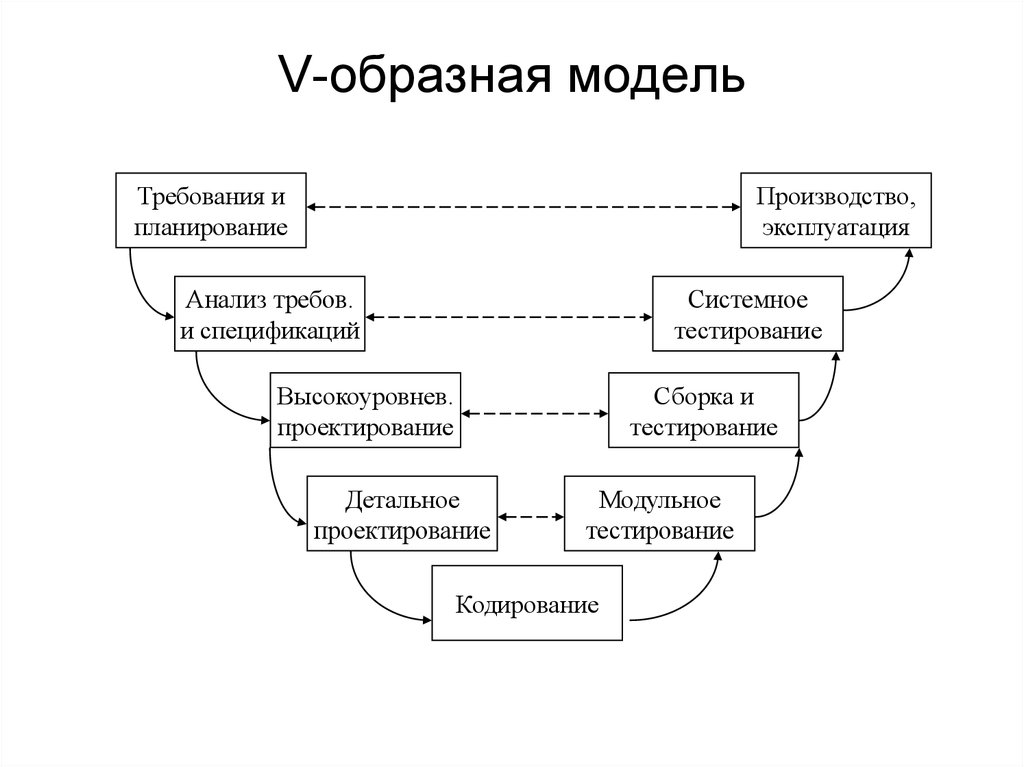
\includegraphics[scale=0.8]{res/v-model.png}
            \caption{V модель разработки ПО}
        \end{center}
    \end{figure}

    Данная модель состоит из двух главных компонентов верификация и валидация. Левая ветка это "--- верификация, а правая "--- валидация.


    \begin{center}
        \textbf{Инкрементная модель}    
    \end{center}

    В данной модели сначала создается базовая функциональность ПО (MVP), затем добавляются доп возможности, и тд проект разрастается. В ходе разработки каждого инкремента у нас получается отдельное работоспособное ПО. Каждый инкремент заранее определен. Подходит, когда есть четкий план развития продукта.

    \begin{figure}[H]
        \begin{center}
            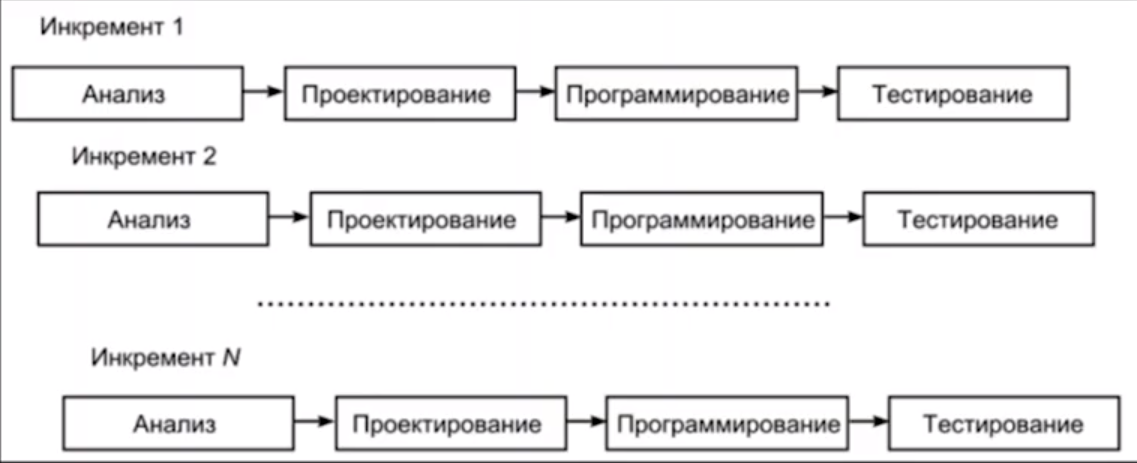
\includegraphics[scale=0.4]{res/increment.png}
            \caption{Инкрементная модель разработки ПО}
        \end{center}
    \end{figure}

    \begin{center}
        \textbf{Итерационная модель}    
    \end{center}

    Каждая новая версия также работоспособная, как и в инкрементной. Но тут мы заранее не знаем, какой будет следующая итерация. Мы смотрим на отзывы пользователей и прочии параметры и отталкиваясь от них решаем, что будет разрабатываться на следующей итерации. Подходит, когда планируется очень долгий проект, который будет разрабатываться не один год.
    
    \begin{figure}[H]
        \begin{center}
            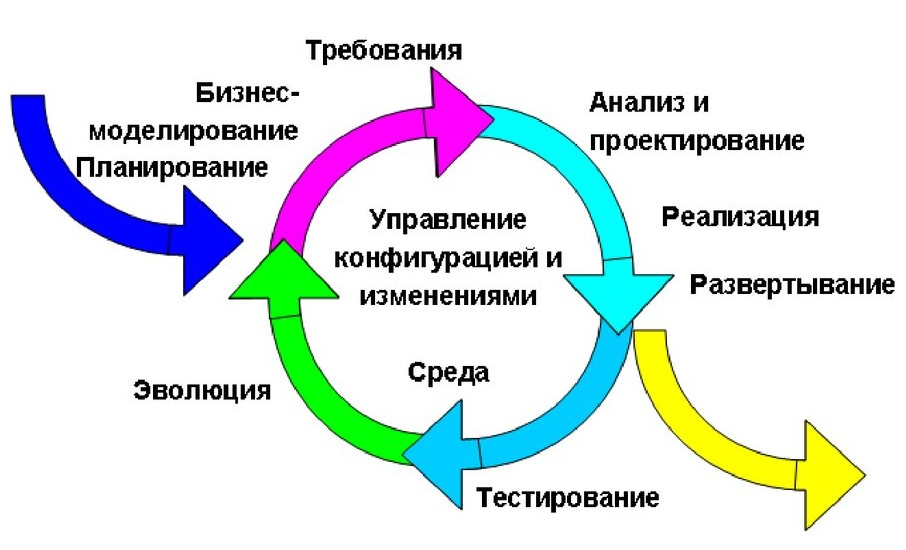
\includegraphics[scale=0.4]{res/iter-model.png}
            \caption{Итерационная модель разработки ПО}
        \end{center}
    \end{figure}

    
    \begin{center}
        \textbf{Спиральная модель}    
    \end{center}
    
    Спиральная модель отличается тем, что на каждой итерации происходит анализ рисков. Также на любом этапе можно отказаться от разработки и выкинуть в релиз то, что есть сейчас. Хорошо подходит для разработки больших проектов, в которых не совсем понятно, к чему стремится продукт.

    \begin{figure}[H]
        \begin{center}
            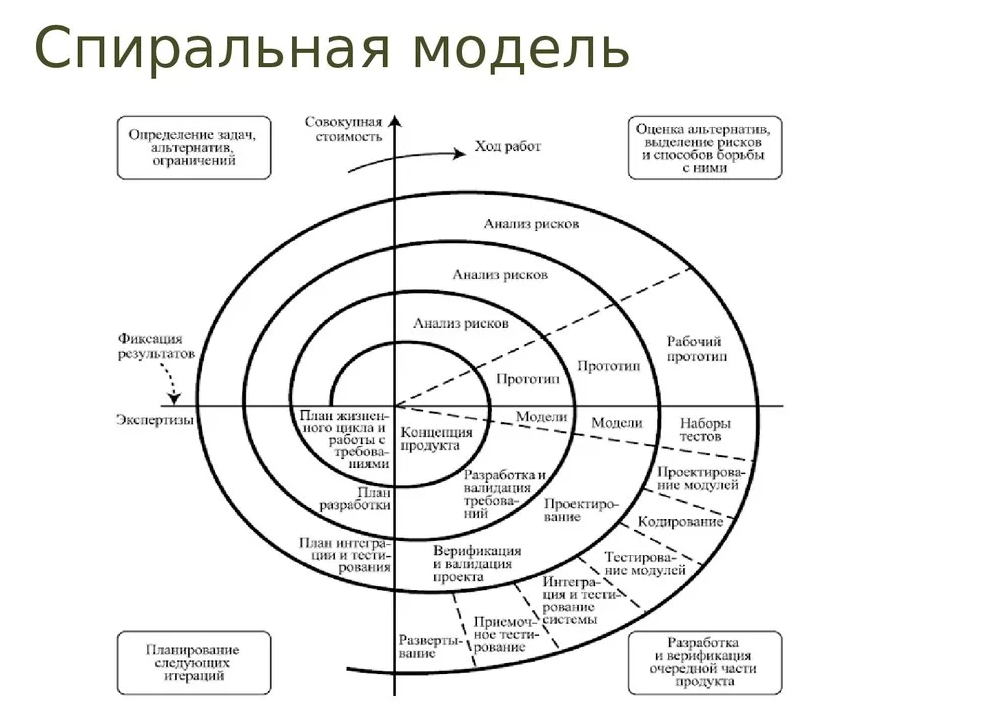
\includegraphics[scale=0.6]{res/spiral-model.png}
            \caption{Спиральная модель разработки ПО}
        \end{center}
    \end{figure}

    \begin{center}
        \textbf{RAD модель}    
    \end{center}
    
    \begin{definition}
        \textbf{RAD (Rapid Application Development model)} "--- быстрая разработка предложений. Отличается тем, что различные модули разрабатываются различными командами, жесткое ограничение времени, различные модули интегрируются в один. Часто используется автоматическая сборка и генерация кода.
    \end{definition}

    Этапы:

    \begin{itemize}[label=$\bullet$]
        \item Бизнес "= моделирование
        \item Анализ и создание модели данных
        \item Анализ и создание процесса
        \item Автоматическая сборка приложения
        \item Тестирование
    \end{itemize}


    \begin{center}
        \textbf{Agile модель}    
    \end{center}

    Это семейство гибких методологий разработок для которых характерно:

    \begin{itemize}[label=$\bullet$]
        \item Короткие итерации
        \item Разные метрики качества работы
        \item Много разных конкретных подходов
    \end{itemize}

    Данный подход рисково использовать для крупных проектов, тк сроки тут явно не указаны.

    Примеры: Канбан, Scrum и тд.

    Agile "= манифест:

    \begin{itemize}[label=$\bullet$]
        \item \textcolor{green}{люди и взаимодействие} важнее \textcolor{red}{процессов и инструментов}
        \item \textcolor{green}{работающий продукт} важнее \textcolor{red}{хорошей документации}
        \item \textcolor{green}{сотрудничество с заказчиком} важнее \textcolor{red}{условий контракта}
        \item \textcolor{green}{готовность к изменениям} важнее \textcolor{red}{первоначального плана}
    \end{itemize}

    \textbf{На разных этапах разработки могут использоваться различные методологии.}

    \section{Continuous integration}
    
    
    \textbf{Continuous Integration} — это практика разработки программного обеспечения, которая заключается в слиянии рабочих копий в общую основную ветвь разработки несколько раз в день и выполнении частых автоматизированных сборок проекта для скорейшего выявления потенциальных дефектов и решения интеграционных проблем. В обычном проекте, где над разными частями системы разработчики трудятся независимо, стадия интеграции является заключительной.

    \begin{figure}[H]
        \begin{center}
            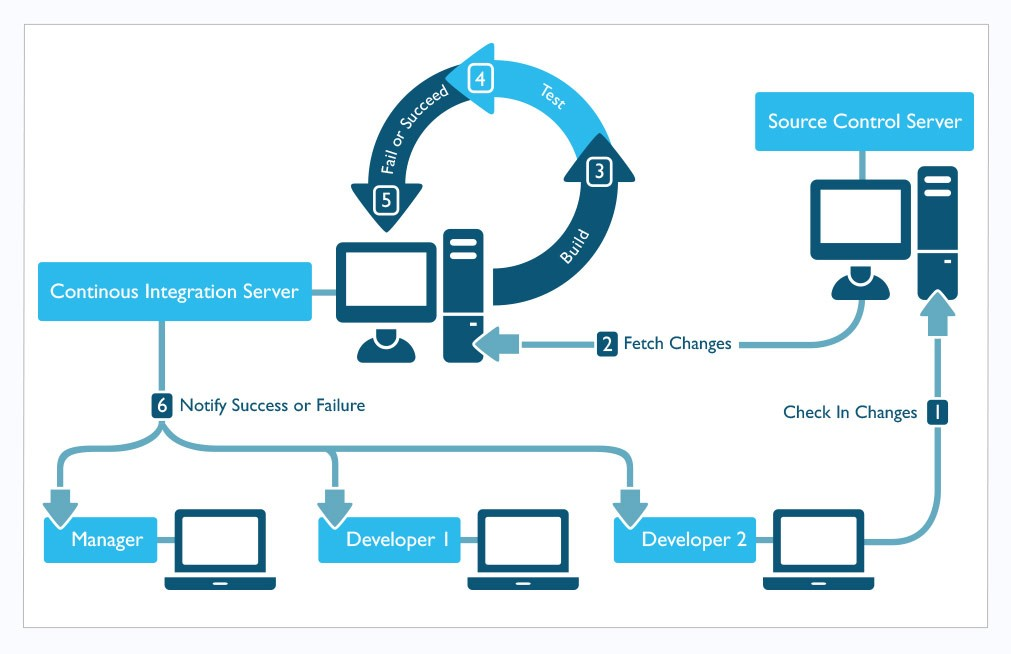
\includegraphics[scale=0.7]{res/ContinuousIntegration.png}
            \caption{Continuous integration}
        \end{center}
    \end{figure}

    Проще говоря, девелоперы трудятся на своих ветках, после того как заливается комит на сервер или в определенное время (к примеру ночью, тк сборка проекта может занять много времени) все ветки собираются в одну, и происходит билд проекта и тестирование. Если билд или тестирование произошло с ошибкой девелоперам, которые делали комит или ответственным за качество сотрудникам отправляется оповещение и они сразу идут его исправлять.

    \textbf{Continuous Delivery} "--- расширяет понятие Continuous Development тем, что помимо обычных тестов, проходит проверка по сценарным тестам.

    \textbf{Continuous Deployment} "--- еще большее расширение, тк если комит прошел все тесты успешно, то сборка выкладывается в продакшен. (Достаточно рисковая практика)
    
    Как выглядит этап сдачи задачи в проекте:
    \begin{enumerate}
        \item  Код-ревью
        \item Исправить имеющиеся замечания, вернуться в п.1
        \item Подготовка краткой документации по задачи
        \item Отправка задачи на независимую проверку (человек получает готовую сборку и краткую документацию пользователя)
        \item Финальный "OK" на готовность влить задачу в ствол проекта
        \item Вливание в ствол 
        \item Задача закрыта
    \end{enumerate}

    \begin{definition}
        \textbf{Мажорная версия} "--- версия, которая будет достаточно долго поддерживаться. (Будут исправляться ошибки, независимо от выхода новых версий)   
    \end{definition}



    \section{Антипаттерны}
    
    Где встречаются антипаттерны:

    \begin{itemize}[label=$\bullet$]
        \item в ООП 
        \item в кодировании
        \item в методологиях
        \item в управлении конфигурацией
    \end{itemize}

    \begin{center}
        \textbf{Антипаттерны в ООП}
    \end{center}

    \textbf{Наследования функциональности от класса утилита, вместо ее делегирования.}
    
    \textbf{Anemic Domain Problem} "--- боязнь размещать логику в объектах предметной области (создавать движок, чтобы он крутил колеса машине, а не сделать так, чтобы колеса крутились сами).
    
    \textbf{Вызов предка} "--- для реализации функциональности методу потомка приходится вызывать те же методы родителя.
    
    \textbf{Ошибка пустого подкласса} "--- когда класс обладает различным поведением по сравнению с классом, который от него наследуется без изменений.
    
    \textbf{God object} "--- концентрация слишком большого количества функциональности в одном классе / модуле / системе
    
    \textbf{Объектная клоака} "--- переиспользование объектов находящихся в непригодном для переиспользования состояние.
    
    \textbf{Полтергейст} "--- объект, чье единственное назначение передавать данные другим объектам.
    
    \textbf{Проблема йо"=йо} "--- чрезмерная размытость сильно связанного кода по иерархии классов.
    
    \textbf{Одиночка} "--- неуместное использование паттерна Singleton.
    
    \textbf{Приватизация} "--- чрезмерное скрытие функциональности, что затрудняет расширение при наследование.
    
    \textbf{Френд"=зона} "--- неуместное использование дружественных классов и функций
    
    \textbf{Каша из интерфейсов} "--- Объединение нескольких интерфейсов, предварительно разделенных, в один.
    
    \textbf{Висячие концы} "---интерфейс, большая часть методов которого пустышки.
    
    \textbf{Заглушка} "--- попытка натянуть малоподходящий интерфейс на класс.

    \begin{definition}
        \textbf{Singleton} "--- класс, для которого создается только один объект.
    \end{definition}



    \begin{center}
        \textbf{Антипаттерны в кодирование}
    \end{center}

    \textbf{Ненужная сложность кода.}
    
    \textbf{Действие на расстояние} "--- взаимодействие между широко разнесенными частями.
    
    \textbf{Накопить и запустить} "--- установка параметров в глобальных переменных.
    
    \textbf{Слепая вера} "--- недостаточная проверка корректности и полноты исправления ошибки или результата работы.
    
    \textbf{Лодочный якорь} "--- сохранение неиспользуемой части кода.
    
    \textbf{Активное ожидание} "--- потребление ресурсов в процессе ожидания запроса, путем выполнения проверок, чтения файлов и тд., вместо асинхронного программирования.
    
    \textbf{Кэширование ошибки} "--- не сбрасывание флага ошибки после ее обработки.
    
    \textbf{Воняющий подгузник} "--- сброс флага ошибки без ее обработки или передачи на уровень выше.
    
    \textbf{Проверка типа вместо интерфейса} "--- проверка на специфический тип, вместо требуемого определенного интерфейса.
    
    \textbf{Инерация кода } "--- избыточное ограничение из-за подразумевания постоянной ее работы в других частях системы (к примеру, убрать из всей системы поддержку 120гц, из-за того, что на телефонах не поддерживается 120гц)
    
    \textbf{Кодирование путем исключения} "--- добавление нового кода для каждого нового особого случая.
    
    \textbf{Таинственный код} "--- использование аббревиатур / сокращений вместо логичных имен.
    
    \textbf{Жесткое кодирование} "--- внедрение предположений в слишком большое количество точек системы.
    
    \textbf{Мягкое кодирование} "--- настраивается вообще все, что усложняет конфигурирование.
    
    \textbf{Поток лавы} "--- сохранение нежелательного кода из-за боязни последствий его удаления / исправления.
    
    \textbf{Волшебные числа} "--- использование числовых констант без объяснения их смысла.
    
    \textbf{Процедурный код} "--- когда стоило отказаться от ООП.
    
    \textbf{Спагетти код} "--- код с чрезмерно запутанным порядком выполнения.
    
    \textbf{Лазанья код} "--- использование неоправданного большого уровней абстракций.
    
    \textbf{Равиоли код} "--- объекты настолько склеены между собой, что невозможно провести рефакторинг.
    
    \textbf{Мыльный пузырь} "--- объект, инициализированный мусор (неинициализированный) слишком долго ведет себя как корректный.

    \textbf{Мьютексный ад} "--- внедрение слишком большого количества примитивов синхронизации в код. 
    
    \textbf{Шаблонный рак} "--- использование шаблонов везде, где можно, а не нужно.



    \begin{center}
        \textbf{Антипаттерны в кодирование}
    \end{center}

    \textbf{Использование паттернов} "--- значит имеется недостаточный уровень абстракции.

    \textbf{Копирование / вставка} "--- нужно делать более общий код.

    \textbf{Дефакторинг} "--- процесс уничтожения функциональности и замена ее документацией.

    \textbf{Золотой молоток} "--- использование любимого решения везде, где только получилось.

    \textbf{Фактор невероятности} "--- гипотеза о том, что известная ошибка не случится.

    \textbf{Преждевременная оптимизация} "--- оптимизация при недостаточной информации.

    \textbf{Метод подбора} "--- софт разрабатываемый путем небольших изменений.

    \textbf{Изобретение велосипеда} "--- создание с нуля того, для чего есть готовое решение.

    \textbf{Изобретение квадратного колеса} "--- создание плохого решения, когда уже есть хорошее готовое.

    \textbf{Самоуничтожение} "--- мелкая ошибка приводит к фатальной.

    \textbf{Два тоннеля} "--- вынесение нового функционала в отдельное приложение.

    \textbf{Коммит убийца} "--- внесение изменений без проверки влияния на другие части программы.

    \textbf{Ад зависимостей} "--- разрастание зависимостей до такого уровня, что раздельная установка / удаление становится затруднительным / невозможным.

    \textbf{Дым и зеркала} "--- демонстрация того, как будут работать еще ненаписанные функции.

    \textbf{Раздувание ПО} "--- разрешение последующим версиям использовать все больше и больше ресурсов.

    \textbf{Функция для галочки} "--- превращение программы в "сборную солянку" плохо работающих и не связанных между собой функций.

    \section{Методы защиты ПО}

    \begin{definition}
        \textbf{Критическая секция} "--- часть кода, которую очень важно защитить. К примеру, модуль авторизации пользователей.
    \end{definition}

    \textbf{Атака}: дизасемблирование "--- получение из исполняемого бинарного файла исходного кода программы.  
    
    \textbf{Защита}: 

    \begin{itemize}[label=$\bullet$]
        \item обфускация исходного кода
        \item шифрование программного кода 
        \item динамическое шифрование (шифрование разных частей кода)
        \item многопроходная расшифровка (те шифрование несколько раз)
        \item архивирование 
        \item динамическое изменение кода программы
        \item использование нестандартной структуры программы
    \end{itemize}
    \hfill \break

    \textbf{Атака}: работа под контролем отладчика (точка останова, которые появляются путем внесения кода 0xCC, которое вызывает прерывание int 3).
    
    \textbf{Защита}:

    \begin{itemize}[label=$\bullet$]
        \item подсчет контрольных сумм программного кода
        \item использование контрольного сумм для расшифровки
        \item многопроходная расшифровка
        \item использование корректирующего кода для поиска контрольного байта (проверка того, что все байты кода находятся на своих местах)
        \item контроль абсолютной времени выполнения
        \item контроль относительного времени выполнения
        \item самостоятельный перехват прерывания
        \item полностью забивать стек критическими данными 
    \end{itemize}
    \hfill \break

    \textbf{Атака}: работа под трассировкой.
    
    \textbf{Защита}: те же самые методы, как и в работе под контролем отладчика.

    \hfill \break
    \hfill \break
    \begin{center}
        \textbf{Защита от нелегального использования}
    \end{center}

    \textbf{Локальная программная защита:} 

    \begin{itemize}[label=$\bullet$]
        \item код на коробке с диском (легко обходится)
    \end{itemize}

    \textbf{Сетевая программная защита:} 
    
    \begin{itemize}[label=$\bullet$]
        \item локальная (в пределах одной сети, если на двух устройствах один и тот же код, то он перестает работать)
        \item глобальная, то же самое, только с удаленным сервером контроля
    \end{itemize}
    Минусы в том, что никто не отменял создания нелегальных серверов.

    \textbf{Защита с помощью аппаратных средств:}
    
    \begin{itemize}[label=$\bullet$]
        \item USB флешки
        \item компакт диски
        \item специальные аппаратные средства (HASH ключи)
        \item привязка лицензии к разнообразным параметрам пк.
    \end{itemize}


    \section{Полезные утилиты}

    Google Test Framework "--- \href{https://google.github.io/googletest/primer.html}{https://google.github.io/googletest/primer.html}
    
    gRPC "--- \href{https://grpc.io/}{https://grpc.io/}

    ПО для Continuous Integration "--- \href{https://www.jenkins.io/}{https://www.jenkins.io/}
    
    ПО для Continuous Integration "--- \href{https://www.travis-ci.com/}{https://www.travis-ci.com/}

\end{document}